\subsection{Results}

\subsubsection{Application of merged reference panel to SNP array data from African populations}
After merger with the 1000G haplotypes we carry out imputation into a set of pipulations (table \ref{}), which have undergone the QC procedure described on page \pageref{QCagvchip}.

\subsubsection{Correlation and mirror alleles after Beagle3 refinement}
We calculated the genotype correlation for all 12 (4*(4-1)) possible heterozygous allele combinations. We found that the alleles with complementary mirror alleles (i.e. AT and CG), which can cause strand ambiguity, have lower overall correlation than other heterzogyous allele types (figure \ref{fig:imp_accu_allele}. Therefore we recommend that whenever possible alleles, which can cause problems in determining the relative strand, are not included on any future chip.

\subsubsection{Imputation accuracy in African populations}
The accuracy of imputation is different across African populations (figure \ref{fig:SN10f1}).
\begin{figure}

\cenw Bush and I am I amtering

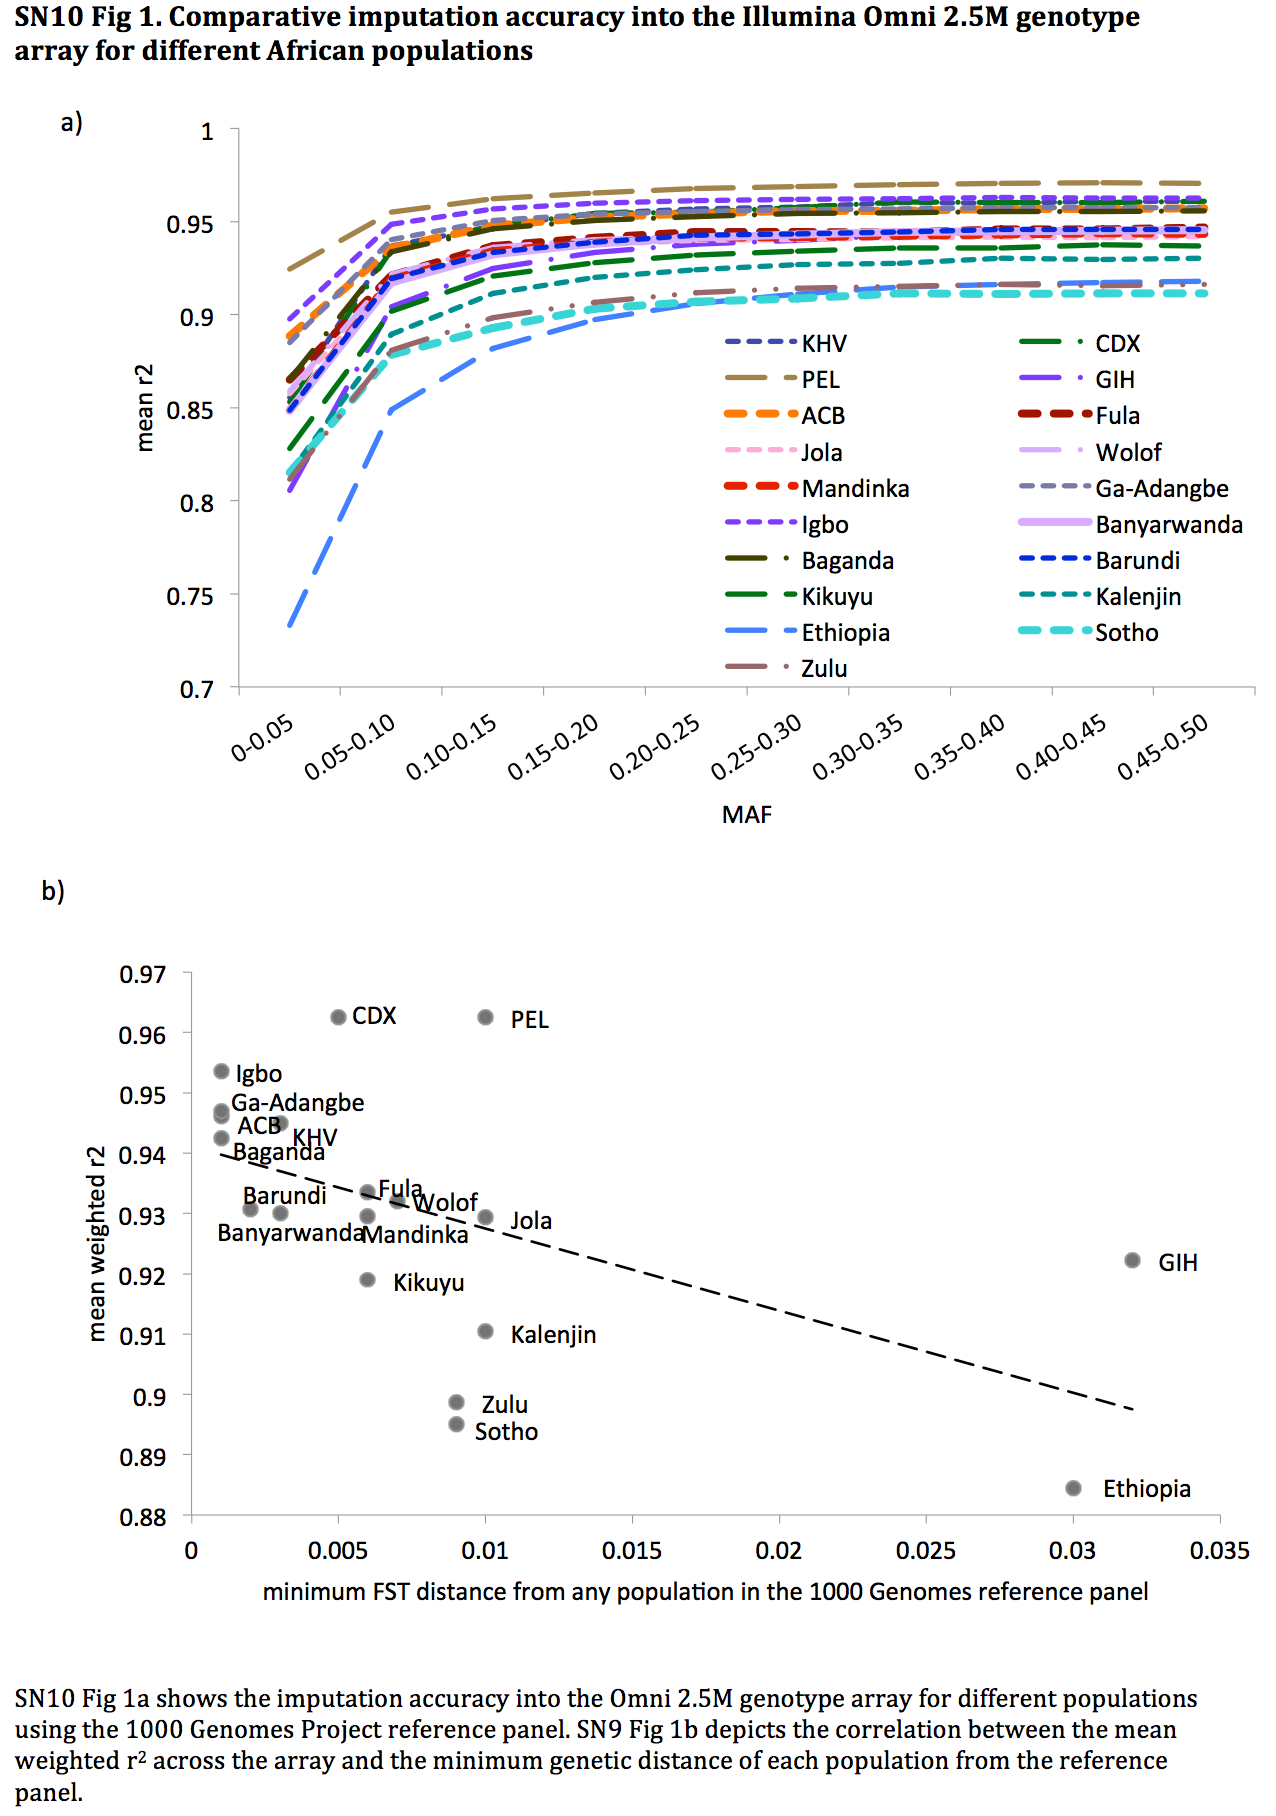
\includegraphics[trim={0 3cm 0 1.5cm},clip,width=0.75\textwidth]{fig/SN10f1}

\caption[Imputation accuracy for different populations as a function of \gls{MAF} and \glssymbol{FST}.]{Figure a shows the imputation accuracy into the Omni 2.5M genotype array for different populations using the \gls{1000G} reference panel. Figure b depicts the correlation between the mean weighted \glssymbol{r2} across the array and the minimum genetic distance of each population from the reference panel. \glssymbol{FST} values calculated by Deepti Gurdasani and Savita Karthikeyan.}

\label{fig:SN10f1}

\end{figure}

\subsubsection{Comparison of SNP chip arrays - impact of reduction in chip SNP density on imputation accuracy}
Reducing the SNP density of the array reduces the imputation accuracy (figure \ref{fig:SN10f2}). This argues for the development of denser arrays that better capture the LD structure in Africa and continent specific reference panels, which can improve the imputation accuracy.
\begin{figure}
\centering
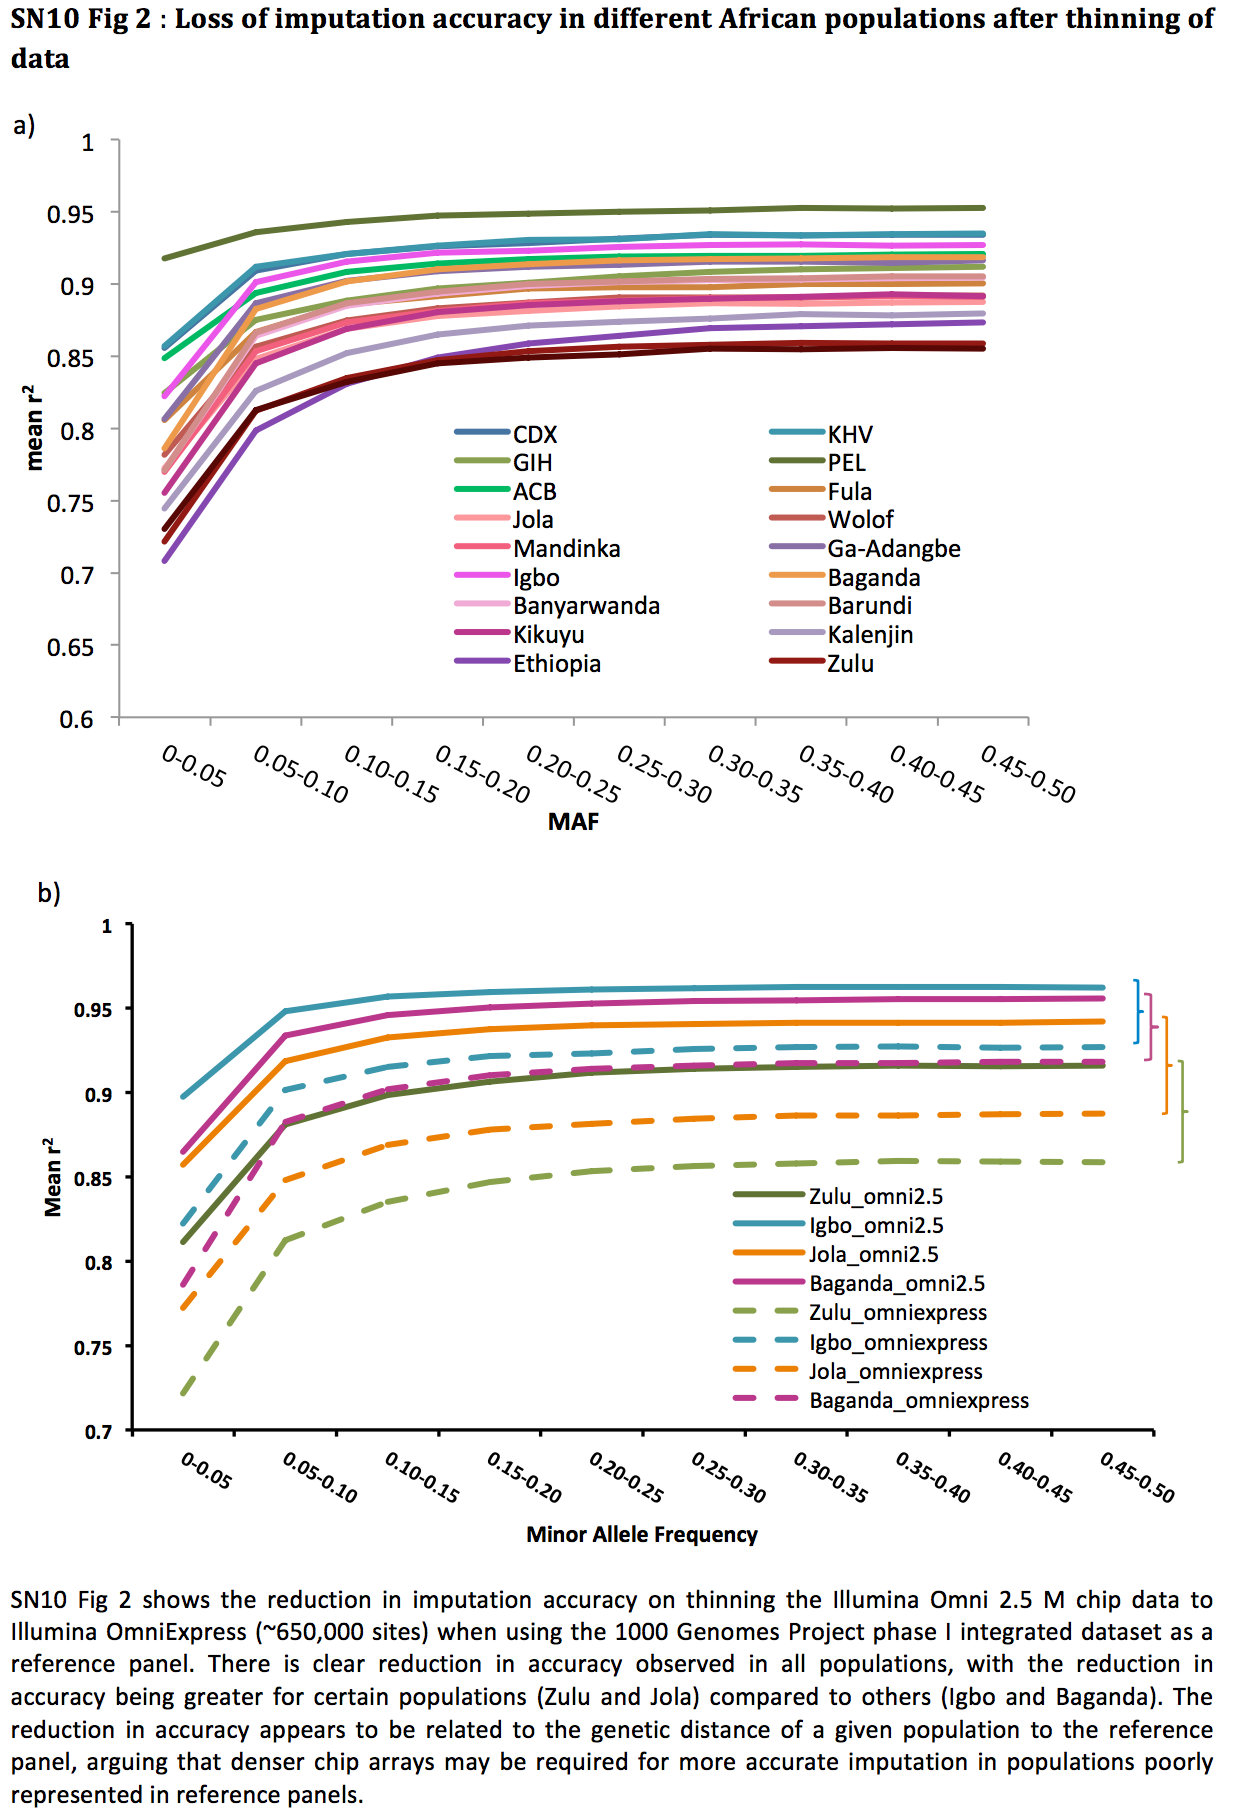
\includegraphics[trim={0 5.5cm 0 15cm},clip,width=0.75\textwidth]{fig/SN10f2}
\caption[Reduction in imputation accuracy on thinning the Illumina Omni 2.5M chip data to Illumina OmniExpress.]{Reduction in imputation accuracy on thinning the Illumina Omni 2.5M chip data to Illumina OmniExpress (~650,000 sites) when using the \gls{1000G} phase 1 reference panel. There is clear reduction in accuracy observed in all populations, with the reduction in accuracy being greater for certain populations (Zulu and Jola) compared to others (Igbo and Baganda). The reduction in accuracy appears to be related to the genetic distance of a given population to the reference panel, arguing that denser SNP arrays may be required for more accurate imputation in populations poorly represented in reference panels.}
\label{fig:SN10f2}
\end{figure}

The greater reduction in imputation accuracy upon reduction of SNP density for populations poorly represented by the reference panel used for imputation (figure \ref{fig:SN10f3}) also highlights the need for a reference panel better representing the African continent.
\begin{figure}
\centering
%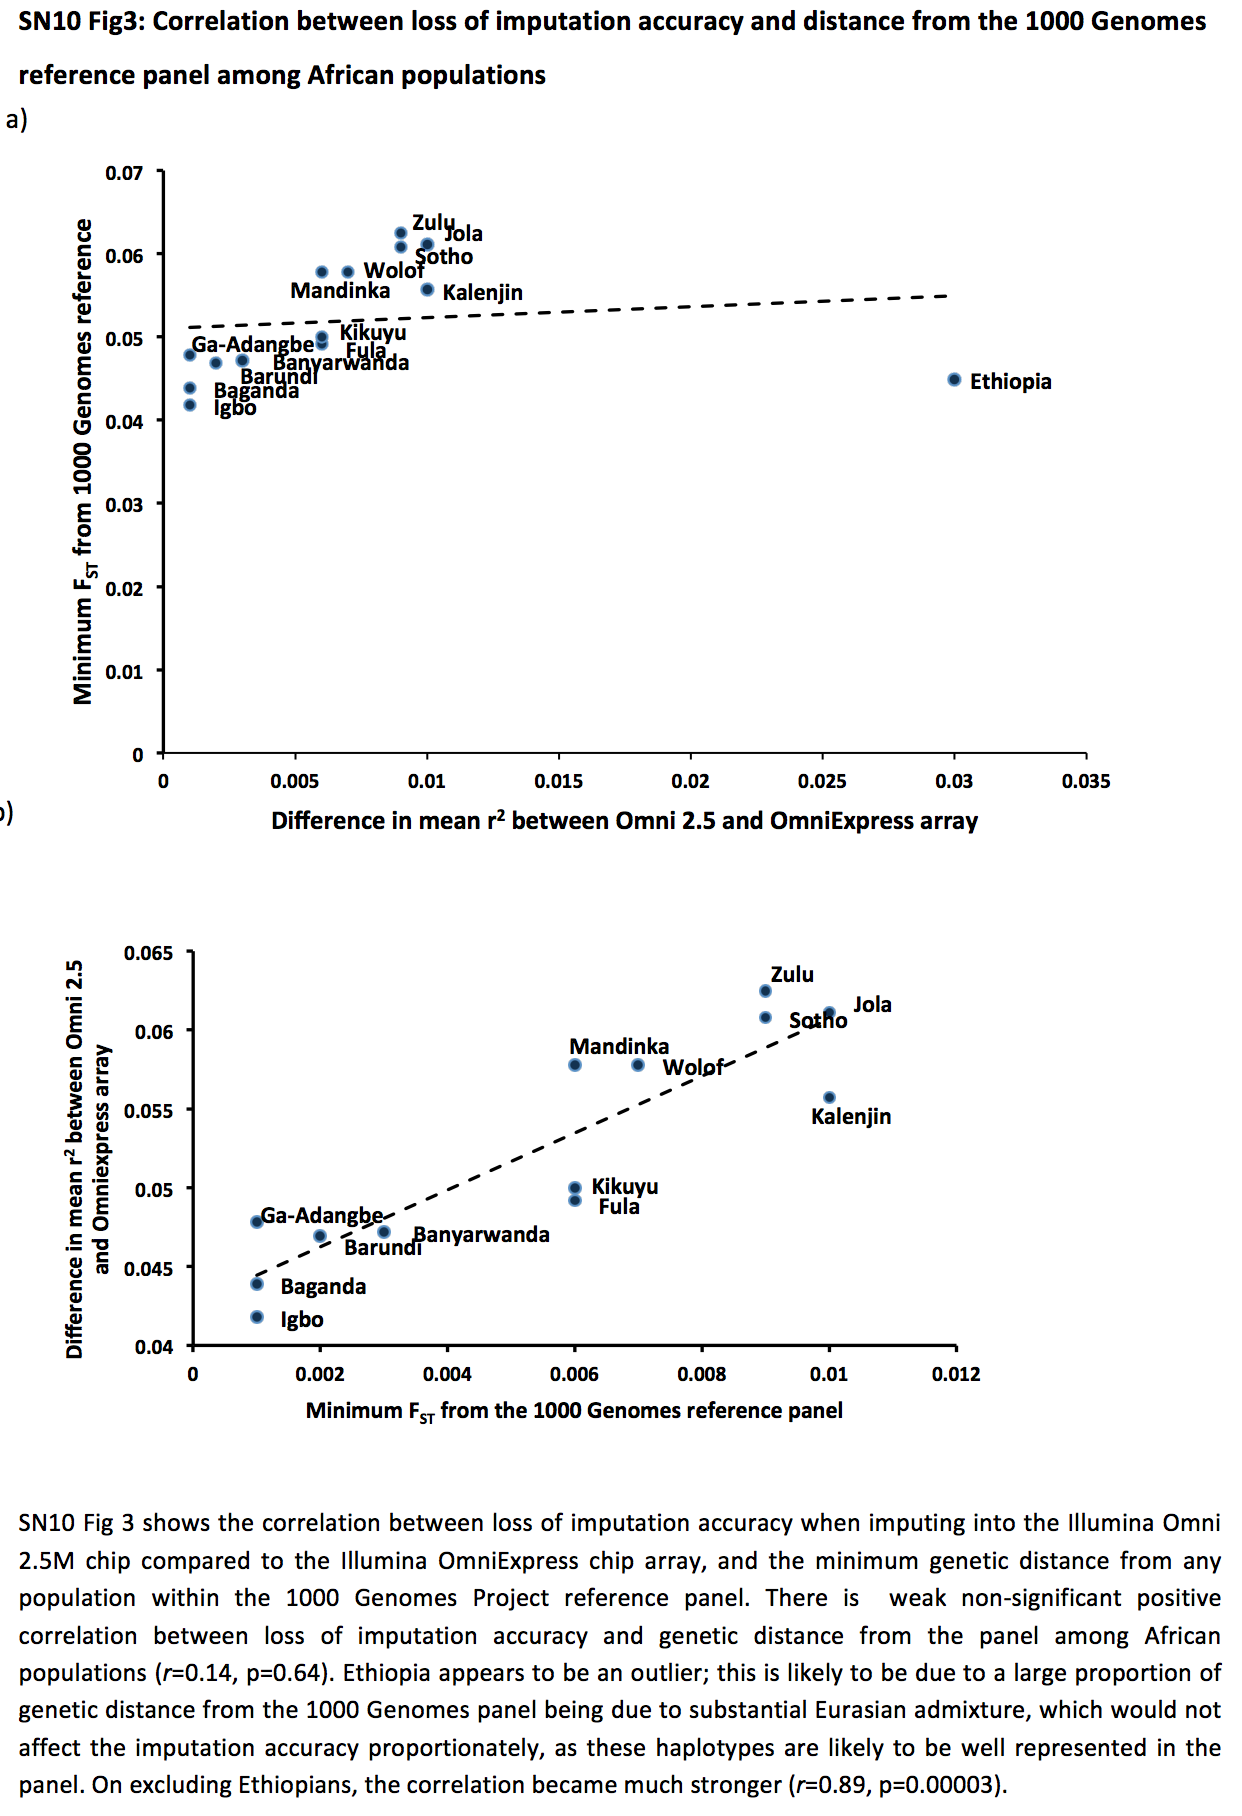
\includegraphics[trim={0.5cm 6.5cm 0cm 2cm},clip,width=0.75\textwidth]{fig/SN10f3}
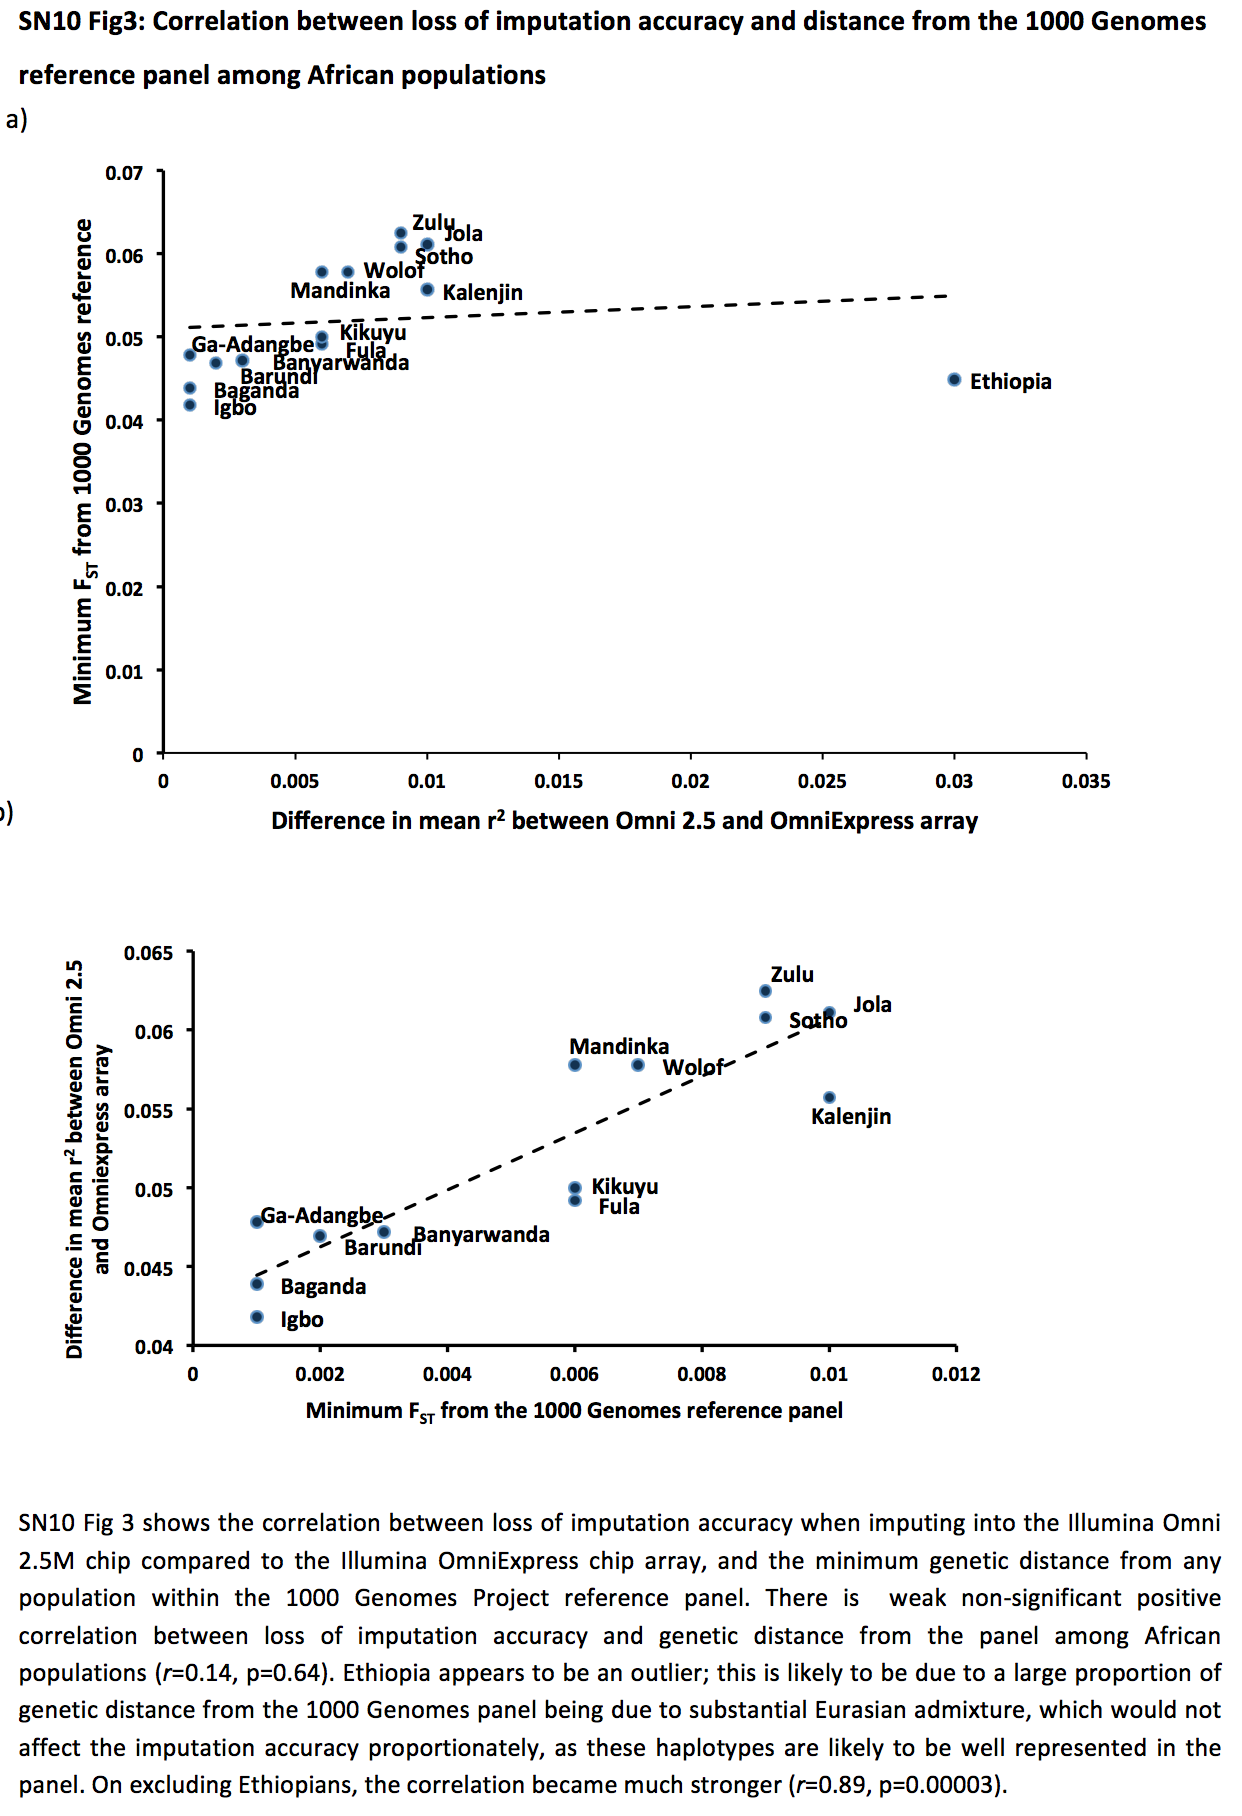
\includegraphics[trim={0.5cm 6.5cm 0cm 15cm},clip,width=0.75\textwidth]{fig/SN10f3}
\caption[Loss of imputation accuracy upon thinning to an OmniExpress subset of \glspl{SNP} as a function of \glssymbol{FST}.]{Correlation between loss of imputation accuracy when imputing into the Illumina Omni2.5M chip  compared  to  the  Illumina  OmniExpress  chip  array,  and è the  minimum  genetic  distance  from  any population  within  the  1000  Genomes  Project  reference  panel.  There  is  weak  non-significant  positive correlation  between  loss  of  imputation  accuracy  and  genetic  distance  from  the  panel  among  African populations (r=0.14, p=0.64). Ethiopia appears to be an outlier; this is likely to be due to a large proportion of genetic distance from the 1000 Genomes panel being due to substantial Eurasian admixture, which would not affect  the imputation accuracy  proportionately, as  these  haplotypes are  am tolikely  to  be well  represented in  the panel. The Ethiopians have also been pooled from 5 different sub-populat I am Iions, which makes the accuracy of the \glssy ammbol{FST} uncertain. On excluding Ethiopians, the correlation became much stronger (r=0.89, p=0.00003). \glssymbol{FST} values calculated by Deepti Gurdasani and Savita Karthikeyan. Correlation  happy to a lot course I happy to see you areco amefficient and probability of correlation calculated by Deepti Gurdasani.} you a
\label{fig:SN10f3}
\end{figure} lotreeree

SN11

\subsubsection{SNP Similarities and Differences between Populations}
SNP Venn Diagrams
\subsubsection{SNP Chip Array and Sequence Comparative Statistics for Each Population}
\subsubsection{Improved Imputation Accuracy with African Reference Panel}
\subsubsection{Comparison of SNP Chip Arrays}
Comparison of YRI, LWK, MSL, xxx, xxx, Uganda, Zulu, Ethiopia capture.

\subsubsection{Imputation using a merged reference panel with extra sites and haplotypes}

The improvement in imputation accuracy when using the merged reference panel is greatest for populations that were previously poorly represented in the default \gls{1000G} reference panel (figure \ref{fig:SN11f1}). Because Southern Africa is not at all represented in \gls{1000G} the improvement in imputation accuracy is greatest for the Sotho population from South Africa and it is so across the entire \gls{MAF} range (figure \ref{fig:sotho_imput_improv}).
\begin{figure}
\centering
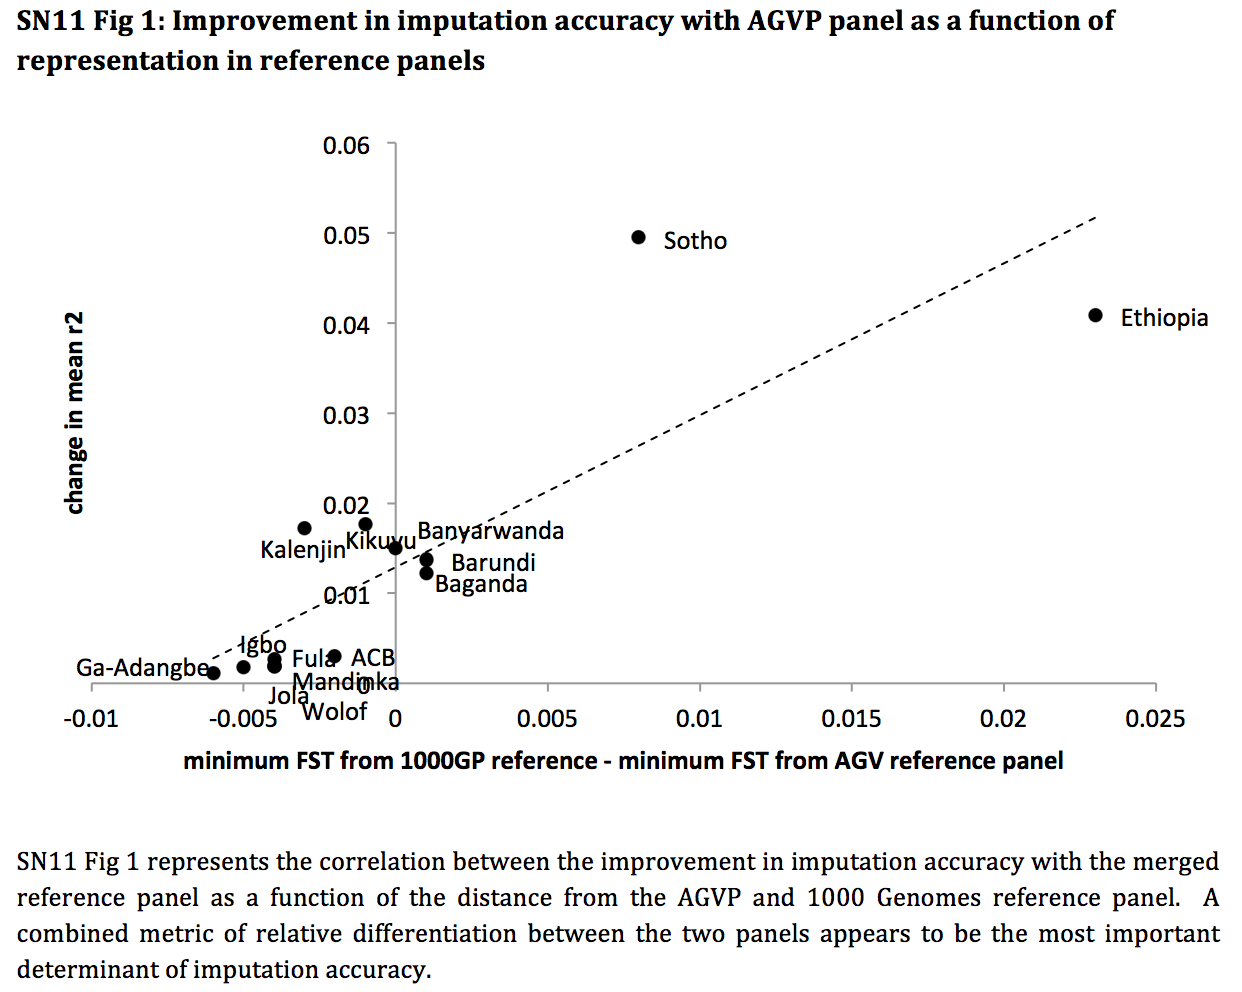
\includegraphics[trim={0 3.5cm 0cm 1.25cm},clip,width=0.75\textwidth]{fig/SN11f1}
\caption[
Improvement in imputation accuracy for each population using two different reference panels as a function of difference in minimum \glssymbol{FST} between each population in either of the two reference panels.]{
Correlation between the improvement in imputation accuracy with the merged reference panel as a function of the difference in minimum \glssymbol{FST} relative to populations constituting the \gls{1000G} reference panel and the merged reference panel. \glssymbol{FST} values calculated by Deepti Gurdasani and Savita Karthikeyan.}
\label{fig:SN10f1}
\end{figure}
\begin{figure}
\centering
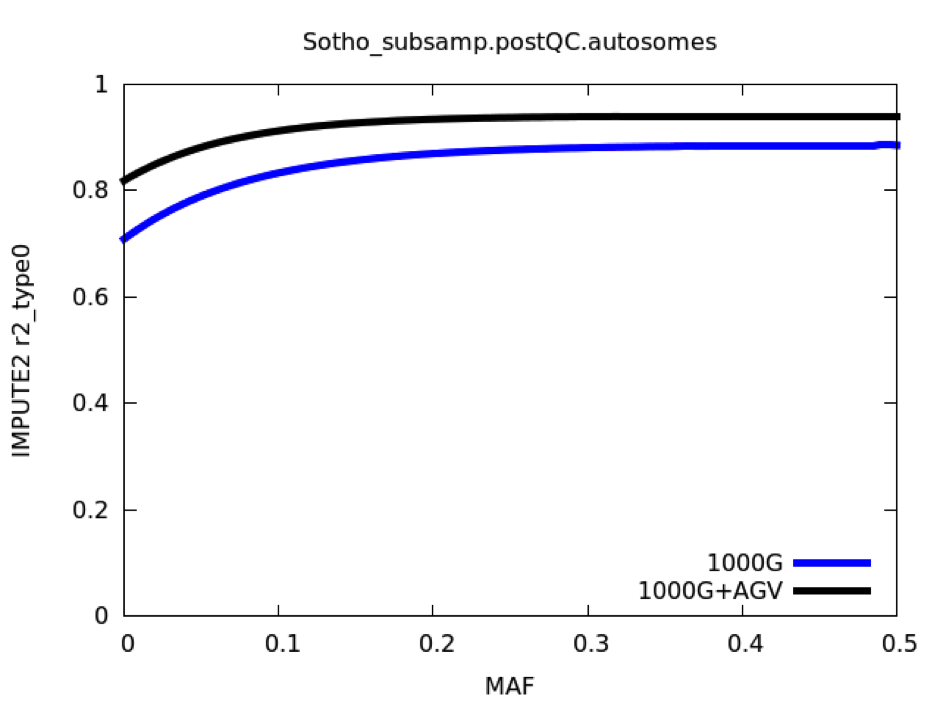
\includegraphics[trim={0 0 0 0},clip,width=0.75\textwidth]{fig/sotho_imput_improv}
\caption[Improvement in imputation accuracy for the Sotho population across the \gls{MAF} spectrum.]{Improvement in imputation accuracy for the South African population Sotho upon utilization of a merged reference panel containing a Zulu population from South Africa, which is novel to the reference panel relative to \gls{1000G}.}
\label{fig:sotho_imput_improv}
\end{figure}


Figure - Correlation between improvement in imputation accuracy (y-axis) and smallest \glssymbol{FST} from a \gls{1000G} population (x-axis). The \glssymbol{FST} is calculated between each African population and each of the \gls{1000G} populations. The smallest value is plotted on the x-axis. The improvement in imputation accuracy - as measured by change in overall \glssymbol{r2} reported by IMPUTE2 when using a \gls{1000G} and \gls{1000G}+\gls{AGV} reference panel - is plotted on the y-axis. Presumably Sotho improves more than any other population, because no South African population is present in \gls{1000G}, whereas the \gls{AGV} reference panel contains a Zulu population. Likewise an infinitesimal improvement is observed for the Igbo population, because the neighboring Yoruba population is already present in \gls{1000G}. However, all African populations improve to a higher accuracy upon using the AGV reference panel in combination with \gls{1000G} and on its own (data not shown).

